% Roofline of the multigrid building blocks on the A100 80GB SXM (FP64).
% Four kernel families: operator evaluation (Laplace apply), restriction,
% prolongation, and the cell-wise smoother.
% Each family has one point per polynomial degree p = 2..5, connected by a line.
% All are memory bound, so the points cluster near the bandwidth slope.
% Two panels: (left) general geometry, (right) Cartesian geometry.
% Transfers (restriction + prolongation) are geometry-independent and identical
%   in both panels (sweep_transf_profile). Operator eval + smoother differ:
%   left panel from sweep_cube_profile2 (Cartesian), right from sweep_ball_profile
%   (general).
%
% Reusable axis style shared by both panels.
\pgfplotsset{
    mg roofline axis/.style={
            width=\linewidth,
            height=0.8\linewidth,
            xlabel={Arithmetic intensity [FLOP/byte]},
            ylabel={Performance [TFLOP/s]},
            log basis x=2,
            xmin=0.25, xmax=16,
            xtick={0.25,0.5,1,2,4,8,16},
            xticklabels={$\frac{1}{4}$,$\frac{1}{2}$,1,2,4,8,16},
            log basis y=2,
            ymin=0.5, ymax=32,
            ytick={0.5,1,2,4,8,16,32},
            yticklabels={$\frac{1}{2}$,1,2,4,8,16,32},
            grid=both,
            legend cell align=left,
            % Common horizontal legend, captured once (on the left panel) and
            % printed above both panels; see \ref{mgrooflinelegend} below.
            legend columns=-1, legend style={/tikz/every even column/.append style={column sep=1em}}, }, }
%
% Rooflines + memory-bound/compute-bound regions, shared by both panels.
\newcommand{\mgrooflinebackground}{%
    % --- Colored regions ---
    % Outer corners are pushed far outside any plausible axis range; only the
    % diagonal boundary points (bandwidth line meets 9.7 at x=4.76 and 19.5 at
    % x=9.56) are physical. pgfplots clips to the axis box, so the same macro
    % renders correctly regardless of each panel's xmin/xmax/ymin/ymax.
    \addplot[green, fill=green, draw=none, fill opacity=0.3, forget plot]
    coordinates {(0.001,0.002039) (4.76,9.7) (1000,9.7) (1000,0.0001) (0.001,0.0001)};
    \addplot[cyan, fill=cyan, draw=none, fill opacity=0.3, forget plot]
    coordinates {(4.76,9.7) (9.56,19.5) (1000,19.5) (1000,9.7)};
    % --- Rooflines: A100 80GB SXM (FP64), bandwidth 2039 GB/s ---
    \addplot[thick, domain=0.001:9.56, samples=2, forget plot] {2.039*x};
    \addplot[thick, domain=0.001:1000, samples=2, forget plot] {9.7};
    \addplot[thick, dashed, domain=0.001:1000, samples=2, forget plot] {19.5};
}
%
% Roofline labels (left panel only). Pinned to fixed data coordinates.
\newcommand{\mgrooflinelabels}{%
    \node[rotate=37.4, above, font=\small\bfseries] at (axis cs:1.2,2.2) {Bandwidth 2039 GB/s};
    \node[above right, font=\small\bfseries] at (axis cs:0.26,9.7) {CUDA 9.7 TFLOP/s};
    \node[above right, font=\small\bfseries] at (axis cs:0.26,19.5) {Tensor 19.5 TFLOP/s};
}
%
% Transfers (geometry-independent), shared by both panels.
\newcommand{\mgrooflinetransfers}{%
    % Restriction (measured, sweep_transf_profile)
    \addplot[red, mark=square*, mark size=2.5pt, thick]
    coordinates {(0.079,0.122) (1.714,2.117) (1.745,1.784) (1.430,1.507)};    % p=2,3,4,5
    \addlegendentry{Restriction}
    % Prolongation (measured, sweep_transf_profile)
    \addplot[orange, mark=diamond*, mark size=2.5pt, thick]
    coordinates {(0.583,0.981) (0.888,1.445) (1.587,2.423) (1.567,2.183)};    % p=2,3,4,5
    \addlegendentry{Prolongation}
}
%
% Common horizontal legend, printed above both panels.
\begin{center}
    \ref{mgrooflinelegend}
\end{center}
%
\begin{minipage}{0.49\linewidth}
    \centering
    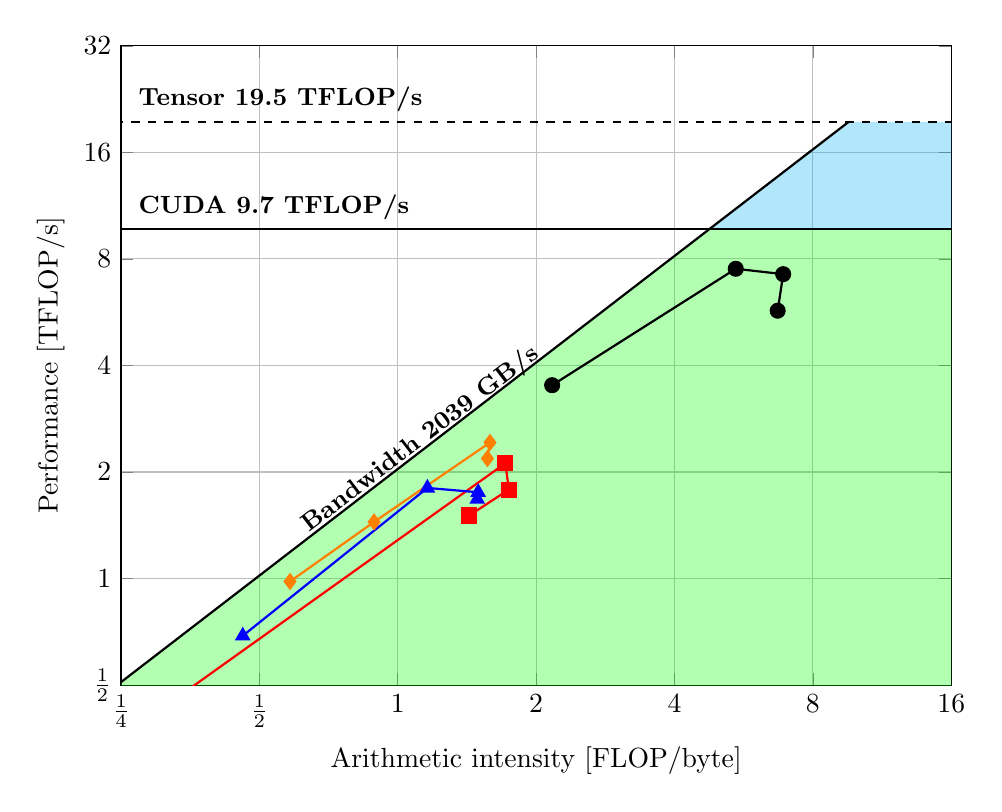
\begin{tikzpicture}
        \begin{loglogaxis}[mg roofline axis, legend to name=mgrooflinelegend]
            \mgrooflinebackground
            \mgrooflinelabels
            % --- Operator evaluation + smoother (Cartesian, sweep_cube_profile2) ---
            \addplot[black, mark=*, mark size=2.5pt, thick]
            coordinates {(2.167,3.518) (5.436,7.503) (6.895,7.245) (6.707,5.711)};      % p=2,3,4,5
            \addlegendentry{Operator eval.}
            \mgrooflinetransfers
            \addplot[blue, mark=triangle*, mark size=2.5pt, thick]
            coordinates {(0.460,0.689) (1.160,1.803) (1.496,1.753) (1.489,1.676)};      % p=2,3,4,5
            \addlegendentry{Smoother}
        \end{loglogaxis}
    \end{tikzpicture}
    {\small Cartesian geometry}
\end{minipage}
\hfill
\begin{minipage}{0.49\linewidth}
    \centering
    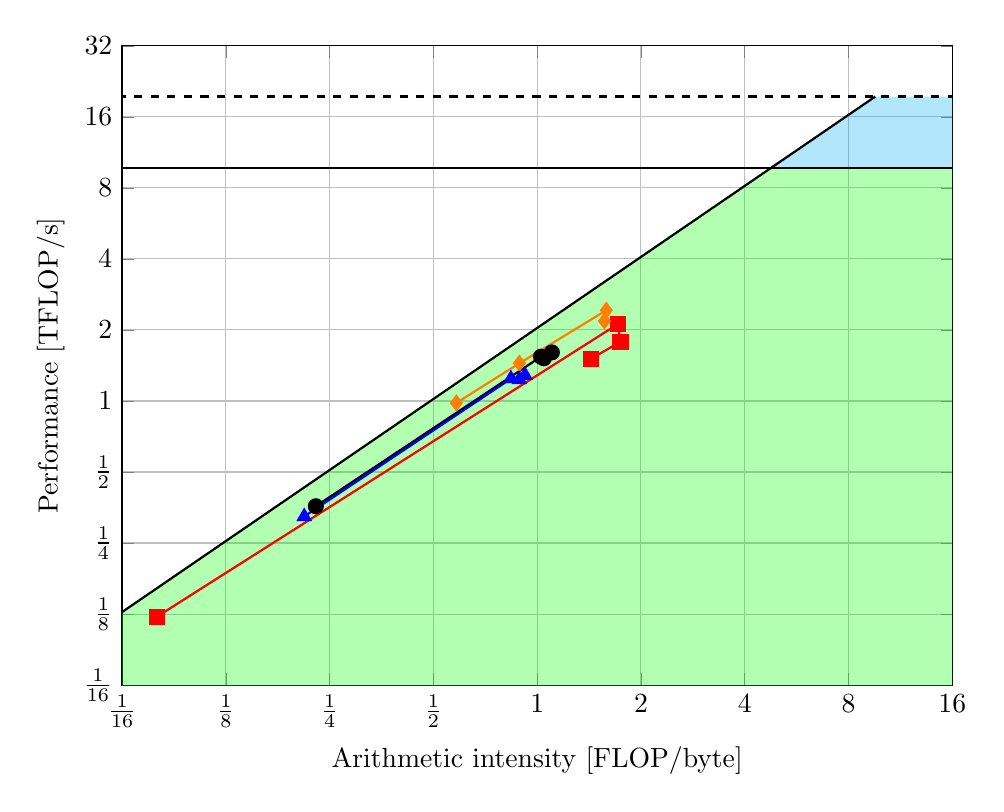
\begin{tikzpicture}
        \begin{loglogaxis}[mg roofline axis, legend to name=mgrooflinelegendunused,
                % General geometry sits low, so drop the axis floor to show all
                % transfer points (incl. the p=2 restriction outlier).
                xmin=0.0625, xtick={0.0625,0.125,0.25,0.5,1,2,4,8,16},
                xticklabels={$\frac{1}{16}$,$\frac{1}{8}$,$\frac{1}{4}$,$\frac{1}{2}$,1,2,4,8,16},
                ymin=0.0625, ytick={0.0625,0.125,0.25,0.5,1,2,4,8,16,32},
                yticklabels={$\frac{1}{16}$,$\frac{1}{8}$,$\frac{1}{4}$,$\frac{1}{2}$,1,2,4,8,16,32}]
            \mgrooflinebackground
            % --- Operator evaluation + smoother (general geometry, sweep_ball_profile) ---
            \addplot[black, mark=*, mark size=2.5pt, thick]
            coordinates {(0.228,0.358) (1.026,1.541) (1.103,1.606) (1.046,1.517)};      % p=2,3,4,5
            \addlegendentry{Operator eval.}
            \mgrooflinetransfers
            \addplot[blue, mark=triangle*, mark size=2.5pt, thick]
            coordinates {(0.211,0.324) (0.839,1.243) (0.922,1.286) (0.888,1.233)};      % p=2,3,4,5
            \addlegendentry{Smoother}
        \end{loglogaxis}
    \end{tikzpicture}
    {\small General geometry}
\end{minipage}
